% hw7.tex

% !TEX program = xelatex
%%%%%%%%%%%%%%%%%%%%
% see http://mirrors.concertpass.com/tex-archive/macros/latex/contrib/tufte-latex/sample-handout.pdf
% for how to use tufte-handout
\documentclass[a4paper, justified]{tufte-handout}

% hw-preamble.tex

% geometry for A4 paper
% See https://tex.stackexchange.com/a/119912/23098
\geometry{
  left=20.0mm,
  top=20.0mm,
  bottom=20.0mm,
  textwidth=130mm, % main text block
  marginparsep=5.0mm, % gutter between main text block and margin notes
  marginparwidth=50.0mm % width of margin notes
}

% for colors
\usepackage{xcolor} % usage: \color{red}{text}
% predefined colors
\newcommand{\red}[1]{\textcolor{red}{#1}} % usage: \red{text}
\newcommand{\blue}[1]{\textcolor{blue}{#1}}
\newcommand{\teal}[1]{\textcolor{teal}{#1}}

\usepackage{todonotes}

% heading
\usepackage{sectsty}
\setcounter{secnumdepth}{2}
\allsectionsfont{\centering\huge\rmfamily}

% for Chinese
\usepackage{xeCJK}
\usepackage{zhnumber}
\setCJKmainfont[BoldFont=FandolSong-Bold.otf]{FandolSong-Regular.otf}

% for fonts
\usepackage{fontspec}
\newcommand{\song}{\CJKfamily{song}}
\newcommand{\kai}{\CJKfamily{kai}}

% To fix the ``MakeTextLowerCase'' bug:
% See https://github.com/Tufte-LaTeX/tufte-latex/issues/64#issuecomment-78572017
% Set up the spacing using fontspec features
\renewcommand\allcapsspacing[1]{{\addfontfeature{LetterSpace=15}#1}}
\renewcommand\smallcapsspacing[1]{{\addfontfeature{LetterSpace=10}#1}}

% for url
\usepackage{hyperref}
\hypersetup{colorlinks = true,
  linkcolor = teal,
  urlcolor  = teal,
  citecolor = blue,
  anchorcolor = blue}

\newcommand{\me}[4]{
    \author{
      {\bfseries 姓名:}\underline{#1}\hspace{2em}
      {\bfseries 学号:}\underline{#2}\hspace{2em}\\[10pt]
      {\bfseries 评分:}\underline{#3\hspace{3em}}\hspace{2em}
      {\bfseries 评阅:}\underline{#4\hspace{3em}}
  }
}

% Please ALWAYS Keep This.
\newcommand{\noplagiarism}{
  \begin{center}
    \fbox{\begin{tabular}{@{}c@{}}
      请独立完成作业,不得抄袭。\\
      若得到他人帮助, 请致谢。\\
      若参考了其它资料,请给出引用。\\
      鼓励讨论,但需独立书写解题过程。
    \end{tabular}}
  \end{center}
}

% \newcommand{\goal}[1]{
%   \begin{center}{\fcolorbox{blue}{yellow!60}{\parbox{0.50\textwidth}{\large
%     \begin{itemize}
%       \item 体会``思维的乐趣''
%       \item 初步了解递归与数学归纳法
%       \item 初步接触算法概念与问题下界概念
%     \end{itemize}}}}
%   \end{center}
% }

% Each hw consists of four parts:
\newcommand{\beginrequired}{\hspace{5em}\section{作业 (必做部分)}}
\newcommand{\beginoptional}{\section{作业 (选做部分)}}
\newcommand{\beginot}{\section{Open Topics}}
\newcommand{\begincorrection}{\section{订正}}
\newcommand{\beginfb}{\section{反馈}}

% for math
\usepackage{amsmath, mathtools, amsfonts, amssymb}
\newcommand{\set}[1]{\{#1\}}

% define theorem-like environments
\usepackage[amsmath, thmmarks]{ntheorem}

\theoremstyle{break}
\theorempreskip{2.0\topsep}
\theorembodyfont{\song}
\theoremseparator{}
\newtheorem{problem}{题目}[subsection]
\renewcommand{\theproblem}{\arabic{problem}}
\newtheorem{ot}{Open Topics}

\theorempreskip{3.0\topsep}
\theoremheaderfont{\kai\bfseries}
\theoremseparator{:}
\theorempostwork{\bigskip\hrule}
\newtheorem*{solution}{解答}
\theorempostwork{\bigskip\hrule}
\newtheorem*{revision}{订正}

\theoremstyle{plain}
\newtheorem*{cause}{错因分析}
\newtheorem*{remark}{注}

\theoremstyle{break}
\theorempostwork{\bigskip\hrule}
\theoremsymbol{\ensuremath{\Box}}
\newtheorem*{proof}{证明}

% \newcommand{\ot}{\blue{\bf [OT]}}

% for figs
\renewcommand\figurename{图}
\renewcommand\tablename{表}

% for fig without caption: #1: width/size; #2: fig file
\newcommand{\fig}[2]{
  \begin{figure}[htbp]
    \centering
    \includegraphics[#1]{#2}
  \end{figure}
}
% for fig with caption: #1: width/size; #2: fig file; #3: caption
\newcommand{\figcap}[3]{
  \begin{figure}[htbp]
    \centering
    \includegraphics[#1]{#2}
    \caption{#3}
  \end{figure}
}
% for fig with both caption and label: #1: width/size; #2: fig file; #3: caption; #4: label
\newcommand{\figcaplbl}[4]{
  \begin{figure}[htbp]
    \centering
    \includegraphics[#1]{#2}
    \caption{#3}
    \label{#4}
  \end{figure}
}
% for margin fig without caption: #1: width/size; #2: fig file
\newcommand{\mfig}[2]{
  \begin{marginfigure}
    \centering
    \includegraphics[#1]{#2}
  \end{marginfigure}
}
% for margin fig with caption: #1: width/size; #2: fig file; #3: caption
\newcommand{\mfigcap}[3]{
  \begin{marginfigure}
    \centering
    \includegraphics[#1]{#2}
    \caption{#3}
  \end{marginfigure}
}

\usepackage{fancyvrb}

% for algorithms
\usepackage[]{algorithm}
\usepackage[]{algpseudocode} % noend
% See [Adjust the indentation whithin the algorithmicx-package when a line is broken](https://tex.stackexchange.com/a/68540/23098)
\newcommand{\algparbox}[1]{\parbox[t]{\dimexpr\linewidth-\algorithmicindent}{#1\strut}}
\newcommand{\hStatex}[0]{\vspace{5pt}}
\makeatletter
\newlength{\trianglerightwidth}
\settowidth{\trianglerightwidth}{$\triangleright$~}
\algnewcommand{\LineComment}[1]{\Statex \hskip\ALG@thistlm \(\triangleright\) #1}
\algnewcommand{\LineCommentCont}[1]{\Statex \hskip\ALG@thistlm%
  \parbox[t]{\dimexpr\linewidth-\ALG@thistlm}{\hangindent=\trianglerightwidth \hangafter=1 \strut$\triangleright$ #1\strut}}
\makeatother

% for footnote/marginnote
% see https://tex.stackexchange.com/a/133265/23098
\usepackage{tikz}
\newcommand{\circled}[1]{%
  \tikz[baseline=(char.base)]
  \node [draw, circle, inner sep = 0.5pt, font = \tiny, minimum size = 8pt] (char) {#1};
}
\renewcommand\thefootnote{\protect\circled{\arabic{footnote}}}

\newcommand{\score}[1]{{\bf [#1 分]}}

\newcommand{\rel}[1]{\xrightarrow{#1}}
\newcommand{\dstar}{\xRightarrow[]{\ast}}
\newcommand{\dplus}{\xRightarrow[]{+}}
\newcommand{\lm}{\xRightarrow[\text{lm}]{}}
\renewcommand{\rm}{\xRightarrow[\text{rm}]{}}
\newcommand{\dpluslm}{\xRightarrow[\text{lm}]{+}}
\newcommand{\dstarlm}{\xRightarrow[\text{lm}]{\ast}}
\newcommand{\dplusrm}{\xRightarrow[\text{rm}]{+}}
\newcommand{\dstarrm}{\xRightarrow[\text{rm}]{\ast}}

\newcommand{\sep}{\;\big\lvert\;}

\newcommand{\first}{\textsc{First}}
\newcommand{\follow}{\textsc{Follow}}

% see https://tex.stackexchange.com/a/109906/23098
\usepackage{empheq}
\newcommand*\widefbox[1]{\fbox{\hspace{2em}#1\hspace{2em}}} % feel free to modify this file if you understand LaTeX well
\usetikzlibrary{shapes.multipart,arrows,automata,positioning}
\newcommand*{\h}{\hspace{15pt}}
\newcommand*{\hg}{\hspace{35pt}}
%%%%%%%%%%%%%%%%%%%%
\title{编译原理作业 (7)}
\me{王腾}{171240540@smail.nju.edu.cn}{}{}
\date{\today}
%%%%%%%%%%%%%%%%%%%%
\begin{document}
\maketitle
%%%%%%%%%%%%%%%%%%%%
\noplagiarism % PLEASE DON'T DELETE THIS LINE!
%%%%%%%%%%%%%%%%%%%%
\begin{abstract}
  % \mfigcap{width = 0.85\textwidth}{figs/George-Boole}{George Boole}
  % \begin{center}{\fcolorbox{blue}{yellow!60}{\parbox{0.65\textwidth}{\large
  %   \begin{itemize}
  %     \item
  %   \end{itemize}}}}
  % \end{center}
\end{abstract}
%%%%%%%%%%%%%%%%%%%%
\beginrequired
%%%%%%%%%%%%%%%

%%%%%%%%%%%%%%%
\begin{problem}[\score{10 = 5 + 5}]
  考虑循环语句
  \[
    \forkw \;(S_{1}; B; S_{2})\; S_{3}
  \]
  \begin{enumerate}[(1)]
    \item 请在控制流语句翻译方案(参考课件或龙书\teal{图 6-36})的基础上为 \forkw{} 语句添加语义规则;
    \item 请为以下代码片段生成中间代码
      \begin{align*}
        &\forkw\; (i = 0; i > 1000 \;\&\&\; i < 2000; i = i + 1) \\
          &\qquad \ifkw\; i == 1225\; \\
          &\qquad\qquad \printkw\; {\textsl{``Merry Christmas''}}
      \end{align*}
      ({\it 注: 最好用图示的方式展示产生式与相应规则的使用情况})
  \end{enumerate}
\end{problem}

\begin{solution}
\begin{enumerate}[(1)]
    \item 语义规则
    
    \begin{tabular}{|l|l|}
        \hline
        \multicolumn{1}{|c|}{产生式}    & \multicolumn{1}{c|}{语义规则}                                                                                                                                                                                                                                            \\ \hline
        $S\to$ \forkw\;($S_1;B;S_2$) $S_3$ 
        & \begin{tabular}[c]{@{}l@{}}
          $S_1.next=newlabel()$\\ 
          $B.true=newlabel()$\\ 
          $B.false=S.next$\\ 
          $S_3.next=newlabel()$\\ 
          $S_2.next=S_1.next$\\ 
          $S.code=S_1.code$ \\ 
          || $label(S_1.next)$ || $B.code$ \\
          || $label(S_3.next)$ || $S_2.code$\\
          || $gen$('goto',$S_1.next$)\\ 
          || $label(B.true)$ || $S_3.code$\\
          || $gen$('goto',$S_3.next$)
        \end{tabular} \\ 
        \hline
        \end{tabular}
    \item $L_i$为标号,假设$S$按顺序产生$L_1(S_1.next),L_2(B.true),L_3(S_3.next)$;\\
    $B$产生$L_4$;$S_3$产生$L_5$。\\
    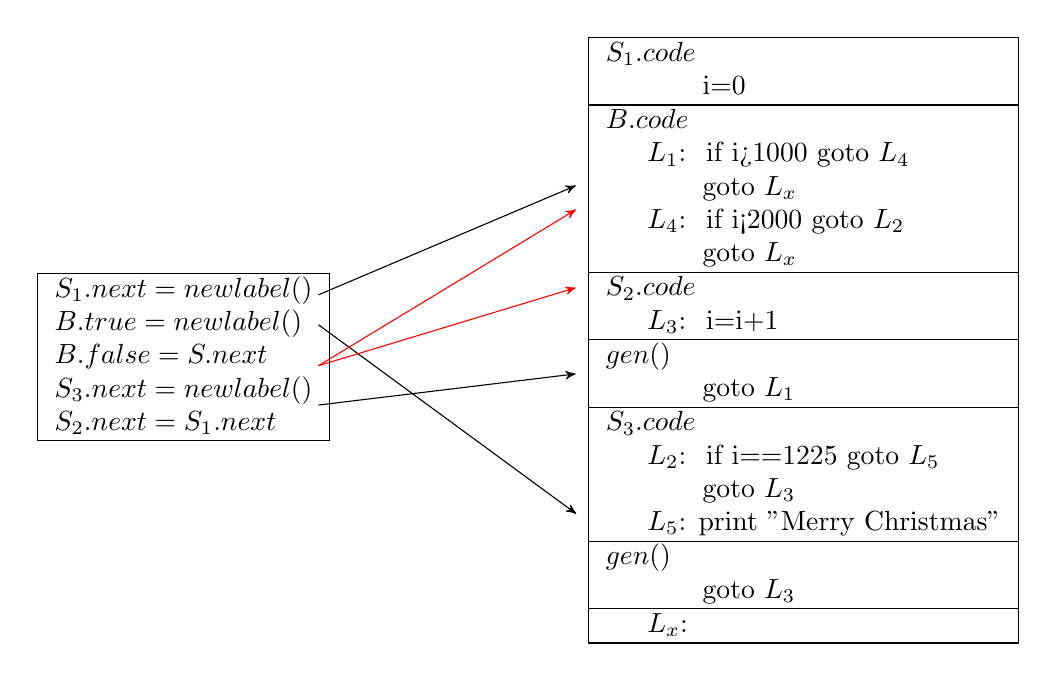
\begin{tikzpicture}[ %可选参数设置此图的属性
        ->, % 有向图
        >=stealth', %箭头末端加粗
        shorten >=1pt, % 箭头末端'>'距终点的距离
        node distance=2cm, % node间最小距离
        on grid, % node中心在网格点上
        scale = 1, %设置网格宽度
        auto % 自动计算位置
      ]
      \tikzstyle{every state}=[fill={rgb:black,1;white,10}] %每个节点填充颜色
      %% node
      % \draw [help lines] (0,0) grid (9,9); % 显示辅助格点位置
      \node[anchor=north west,yshift=6cm] (0) {
        \begin{tabular}{|l|l|}
            \hline
            $S_1.next=newlabel()$\\ $B.true=newlabel()$\\ $B.false=S.next$\\ $S_3.next=newlabel()$\\ $S_2.next=S_1.next$\\ \hline
        \end{tabular}
      };% table
      \node[anchor=north west,xshift=7cm, yshift=9cm] (1) {
        \begin{tabular}{|l|}
          \hline
          \begin{tabular}[c]{@{}l@{}}$S_1.code$\\   \hg i=0\end{tabular}                                                                                                   \\ \hline
          \begin{tabular}[c]{@{}l@{}}$B.code$\\   \h $L_1$:\; if i>1000 goto $L_4$\\   \hg goto $L_x$\\   \h $L_4$:\; if i<2000 goto $L_2$\\   \hg goto $L_x$\end{tabular} \\ \hline
          \begin{tabular}[c]{@{}l@{}}$S_2.code$\\   \h $L_3$:\; i=i+1\end{tabular}                                                                                         \\ \hline
          \begin{tabular}[c]{@{}l@{}}$gen()$\\   \hg goto $L_1$\end{tabular}                                                                                               \\ \hline
          \begin{tabular}[c]{@{}l@{}}$S_3.code$\\   \h $L_2$:\; if i==1225 goto $L_5$\\   \hg goto $L_3$\\   \h $L_5$: print "Merry Christmas"\end{tabular}                      \\ \hline
          \begin{tabular}[c]{@{}l@{}}$gen()$\\   \hg goto $L_3$\end{tabular}                                                                                               \\ \hline
          \h $L_x$:                                                                                                                                                        \\ \hline
          \end{tabular}
      };% table
      %% path
    % \path (0,0) -- (2,0)
    \draw (3.7,5.6) -> (7,7) ; 
    \draw (3.7,5.22) ->  (7,2.8); 
    \draw (3.7,4.2) -> (7,4.6) ; 
    \draw[red] (3.7,4.7) ->  (7,5.7); 
    \draw[red] (3.7,4.7) ->  (7,6.7); 
\end{tikzpicture}
      
        
        
  \end{enumerate}    
\end{solution}
%%%%%%%%%%%%%%%

%%%%%%%%%%%%%%%%%%%%
% 如果没有需要订正的题目,可以把这部分删掉

% \begincorrection
%%%%%%%%%%%%%%%%%%%%

%%%%%%%%%%%%%%%%%%%%
% 如果没有反馈,可以把这部分删掉

%%%%%%%%%%%%%%%%%%%%
\end{document}